% ******************************* PhD Thesis Template **************************
% Please have a look at the README.md file for info on how to use the template

\documentclass[a4paper,12pt,times,numbered,print,index]{Classes/PhDThesisPSnPDF}

% ******************************************************************************
% ******************************* Class Options ********************************
% *********************** See README for more details **************************
% ******************************************************************************

% `a4paper'(The University of Cambridge PhD thesis guidelines recommends a page
% size a4 - default option) or `a5paper': A5 Paper size is also allowed as per
% the Cambridge University Engineering Deparment guidelines for PhD thesis
%
% `11pt' or `12pt'(default): Font Size 10pt is NOT recommended by the University
% guidelines
%
% `oneside' or `twoside'(default): Printing double side (twoside) or single
% side.
%
% `print': Use `print' for print version with appropriate margins and page
% layout. Leaving the options field blank will activate Online version.
%
% `index': For index at the end of the thesis
%
% `draftclassic': For draft mode without loading any images (same as draft in book)
%
% `draft': Special draft mode with line numbers, images, and water mark with
% timestamp and custom text. Position of the text can also be modified.
%
% `abstract': To generate only the title page and abstract page with
% dissertation title and name, to submit to the Student Registry
%
% `chapter`: This option enables only the specified chapter and it's references
%  Useful for review and corrections.
%
% ************************* Custom Page Margins ********************************
%
% `custommargin`: Use `custommargin' in options to activate custom page margins,
% which can be defined in the preamble.tex. Custom margin will override
% print/online margin setup.
%
% *********************** Choosing the Fonts in Class Options ******************
%
% `times' : Times font with math support. (The Cambridge University guidelines
% recommend using times)
%
% `fourier': Utopia Font with Fourier Math font (Font has to be installed)
%            It's a free font.
%
% `customfont': Use `customfont' option in the document class and load the
% package in the preamble.tex
%
% default or leave empty: `Latin Modern' font will be loaded.
%
% ********************** Choosing the Bibliography style ***********************
%
% `authoryear': For author-year citation eg., Krishna (2013)
%
% `numbered': (Default Option) For numbered and sorted citation e.g., [1,5,2]
%
% `custombib': Define your own bibliography style in the `preamble.tex' file.
%              `\RequirePackage[square, sort, numbers, authoryear]{natbib}'.
%              This can be also used to load biblatex instead of natbib
%              (See Preamble)
%
% **************************** Choosing the Page Style *************************
%
% `default (leave empty)': For Page Numbers in Header (Left Even, Right Odd) and
% Chapter Name in Header (Right Even) and Section Name (Left Odd). Blank Footer.
%
% `PageStyleI': Chapter Name next & Page Number on Even Side (Left Even).
% Section Name & Page Number in Header on Odd Side (Right Odd). Footer is empty.
%
% `PageStyleII': Chapter Name on Even Side (Left Even) in Header. Section Number
% and Section Name in Header on Odd Side (Right Odd). Page numbering in footer

% Uncomment to change page style
%\pagestyle{PageStyleII}

% ********************************** Preamble **********************************
% Preamble: Contains packages and user-defined commands and settings
% ******************************************************************************
% ****************************** Custom Margin *********************************

% Add `custommargin' in the document class options to use this section
% Set {innerside margin / outerside margin / topmargin / bottom margin}  and
% other page dimensions
\ifsetCustomMargin
  \RequirePackage[left=37mm,right=30mm,top=35mm,bottom=30mm]{geometry}
  \setFancyHdr % To apply fancy header after geometry package is loaded
\fi

% Add spaces between paragraphs
%\setlength{\parskip}{0.5em}
% Ragged bottom avoids extra whitespaces between paragraphs
\raggedbottom
% To remove the excess top spacing for enumeration, list and description
%\usepackage{enumitem}
%\setlist[enumerate,itemize,description]{topsep=0em}

% *****************************************************************************
% ******************* Fonts (like different typewriter fonts etc.)*************

% Add `customfont' in the document class option to use this section

\ifsetCustomFont
  % Set your custom font here and use `customfont' in options. Leave empty to
  % load computer modern font (default LaTeX font).
  %\RequirePackage{helvet}

  % For use with XeLaTeX
  %  \setmainfont[
  %    Path              = ./libertine/opentype/,
  %    Extension         = .otf,
  %    UprightFont = LinLibertine_R,
  %    BoldFont = LinLibertine_RZ, % Linux Libertine O Regular Semibold
  %    ItalicFont = LinLibertine_RI,
  %    BoldItalicFont = LinLibertine_RZI, % Linux Libertine O Regular Semibold Italic
  %  ]
  %  {libertine}
  %  % load font from system font
  %  \newfontfamily\libertinesystemfont{Linux Libertine O}
\fi

% *****************************************************************************
% **************************** Custom Packages ********************************

% ************************* Algorithms and Pseudocode **************************

%\usepackage{algpseudocode}


% ********************Captions and Hyperreferencing / URL **********************

% Captions: This makes captions of figures use a boldfaced small font.
%\RequirePackage[small,bf]{caption}

\RequirePackage[labelsep=space,tableposition=top]{caption}
\renewcommand{\figurename}{Fig.} %to support older versions of captions.sty


% *************************** Graphics and figures *****************************

%\usepackage{rotating}
%\usepackage{wrapfig}

% Uncomment the following two lines to force Latex to place the figure.
% Use [H] when including graphics. Note 'H' instead of 'h'
%\usepackage{float}
%\restylefloat{figure}

% Subcaption package is also available in the sty folder you can use that by
% uncommenting the following line
% This is for people stuck with older versions of texlive
%\usepackage{sty/caption/subcaption}
\usepackage{subcaption}

% ********************************** Tables ************************************
\usepackage{booktabs} % For professional looking tables
\usepackage{multirow}

%\usepackage{multicol}
%\usepackage{longtable}
%\usepackage{tabularx}


% *********************************** SI Units *********************************
\usepackage{siunitx} % use this package module for SI units


% ******************************* Line Spacing *********************************

% Choose linespacing as appropriate. Default is one-half line spacing as per the
% University guidelines

% \doublespacing
% \onehalfspacing
% \singlespacing


% ************************ Formatting / Footnote *******************************

% Don't break enumeration (etc.) across pages in an ugly manner (default 10000)
%\clubpenalty=500
%\widowpenalty=500

%\usepackage[perpage]{footmisc} %Range of footnote options


% *****************************************************************************
% *************************** Bibliography  and References ********************

%\usepackage{cleveref} %Referencing without need to explicitly state fig /table

% Add `custombib' in the document class option to use this section
\ifuseCustomBib
   \RequirePackage[square, sort, numbers, authoryear]{natbib} % CustomBib

% If you would like to use biblatex for your reference management, as opposed to the default `natbibpackage` pass the option `custombib` in the document class. Comment out the previous line to make sure you don't load the natbib package. Uncomment the following lines and specify the location of references.bib file

%\RequirePackage[backend=biber, style=numeric-comp, citestyle=numeric, sorting=nty, natbib=true]{biblatex}
%\bibliography{References/references} %Location of references.bib only for biblatex

\fi

% changes the default name `Bibliography` -> `References'
\renewcommand{\bibname}{References}


% ******************************************************************************
% ************************* User Defined Commands ******************************
% ******************************************************************************

% *********** To change the name of Table of Contents / LOF and LOT ************

%\renewcommand{\contentsname}{My Table of Contents}
%\renewcommand{\listfigurename}{My List of Figures}
%\renewcommand{\listtablename}{My List of Tables}


% ********************** TOC depth and numbering depth *************************

\setcounter{secnumdepth}{2}
\setcounter{tocdepth}{2}


% ******************************* Nomenclature *********************************

% To change the name of the Nomenclature section, uncomment the following line

%\renewcommand{\nomname}{Symbols}


% ********************************* Appendix ***********************************

% The default value of both \appendixtocname and \appendixpagename is `Appendices'. These names can all be changed via:

%\renewcommand{\appendixtocname}{List of appendices}
%\renewcommand{\appendixname}{Appndx}

% *********************** Configure Draft Mode **********************************

% Uncomment to disable figures in `draft'
%\setkeys{Gin}{draft=true}  % set draft to false to enable figures in `draft'

% These options are active only during the draft mode
% Default text is "Draft"
%\SetDraftText{DRAFT}

% Default Watermark location is top. Location (top/bottom)
%\SetDraftWMPosition{bottom}

% Draft Version - default is v1.0
%\SetDraftVersion{v1.1}

% Draft Text grayscale value (should be between 0-black and 1-white)
% Default value is 0.75
%\SetDraftGrayScale{0.8}


% ******************************** Todo Notes **********************************
%% Uncomment the following lines to have todonotes.

%\ifsetDraft
%	\usepackage[colorinlistoftodos]{todonotes}
%	\newcommand{\mynote}[1]{\todo[author=kks32,size=\small,inline,color=green!40]{#1}}
%\else
%	\newcommand{\mynote}[1]{}
%	\newcommand{\listoftodos}{}
%\fi

% Example todo: \mynote{Hey! I have a note}


% ************************ Thesis Information & Meta-data **********************
% Thesis title and author information, refernce file for biblatex
% ************************ Thesis Information & Meta-data **********************
%% The title of the thesis
\title{Automated User-Generated Content Curation with Deep Learning Techniques}
%\texorpdfstring is used for PDF metadata. Usage:
%\texorpdfstring{LaTeX_Version}{PDF Version (non-latex)} eg.,
%\texorpdfstring{$sigma$}{sigma}

%% Subtitle (Optional)
\subtitle{PhD Thesis Research Plan}

%% The full name of the author
\author{Stalin Leonel Cruz}

%% Department (eg. Department of Engineering, Maths, Physics)
\dept{Department of Computer Architecture}

%% University and Crest
\university{Universitat Politècnica de Catalunya}
% Crest minimum should be 30mm.
\crest{
\includegraphics[width=0.50\textwidth]{dac_logo.jpeg}}
%% Use this crest, if you are using the college crest
%% Crest long miminum should be 65mm
%\crest{
\includegraphics[width=0.45\textwidth]{University_Crest_Long}}

%% College shield [optional] 
% Crest minimum should be 30mm.
%\collegeshield{
\includegraphics[width=0.2\textwidth]{CollegeShields/Kings}}


%% Supervisor (optional)
%% for multiple supervisors, append each supervisor with the \newline command
\supervisor{Dr. Ruben Tous\newline
Dra. Beatriz Otero}

%% Supervisor Role (optional) - Supervisor (default) or advisor
% \supervisorrole{\textbf{Supervisors: }}
%% if no title is desired:
% \supervisorrole{}

%% Supervisor line width: required to align supervisors
%\supervisorlinewidth{0.35\textwidth}

%% Advisor (optional)
%% for multiple advisors, append each advisor with the \newline command
%\advisor{Dr. A. Advisor\newline
%Dr. B. Advisor}
     
%% Advisor Role (optional) - Advisor (default) or leave empty
% \advisorrole{Advisors: }
%% if no title is required
% \advisorrole{}

%% Advisor line width: required to align supervisors
%\advisorlinewidth{0.25\textwidth}


%% You can redefine the submission text:
% Default as per the University guidelines:
% ``This dissertation is submitted for the degree of''
\renewcommand{\submissiontext}{This Research Plan is submitted for the degree of}

%% Full title of the Degree
\degreetitle{Doctor of Philosophy}

%% College affiliation (optional)
\college{Universitat Politècnica de Catalunya}

%% Submission date
% Default is set as {\monthname[\the\month]\space\the\year}
%\degreedate{September 2014} 

%% Meta information
\subject{LaTeX} \keywords{{LaTeX} {PhD Thesis} {Engineering} {Universitat Politècnica de Catalunya}}


% ***************************** Abstract Separate ******************************
% To printout only the titlepage and the abstract with the PhD title and the
% author name for submission to the Student Registry, use the `abstract' option in
% the document class.

\ifdefineAbstract
 \pagestyle{empty}
 \includeonly{Declaration/declaration, Abstract/abstract}
\fi

% ***************************** Chapter Mode ***********************************
% The chapter mode allows user to only print particular chapters with references
% Title, Contents, Frontmatter are disabled by default
% Useful option to review a particular chapter or to send it to supervisior.
% To use choose `chapter' option in the document class

\ifdefineChapter
 \includeonly{Chapter3/chapter3}
\fi

% ******************************** Front Matter ********************************
\begin{document}

\frontmatter

\maketitle

%% ******************************* Thesis Dedidcation ********************************

\begin{dedication} 

I would like to dedicate this thesis to my loving parents \dots

\end{dedication}


%% ******************************* Thesis Declaration ***************************

\begin{declaration}

I hereby declare that except where specific reference is made to the work of 
others, the contents of this dissertation are original and have not been 
submitted in whole or in part for consideration for any other degree or 
qualification in this, or any other university. This dissertation is my own 
work and contains nothing which is the outcome of work done in collaboration 
with others, except as specified in the text and Acknowledgements. This 
dissertation contains fewer than 65,000 words including appendices, 
bibliography, footnotes, tables and equations and has fewer than 150 figures.

% Author and date will be inserted automatically from thesis.tex \author \degreedate

\end{declaration}


%% ************************** Thesis Acknowledgements **************************

\begin{acknowledgements}      


And I would like to acknowledge ...


\end{acknowledgements}

%% ************************** Thesis Abstract *****************************
% Use `abstract' as an option in the document class to print only the titlepage and the abstract.
\begin{abstract}
This is where you write your abstract ...
\end{abstract}


% *********************** Adding TOC and List of Figures ***********************

\tableofcontents

%\listoffigures

%\listoftables

% \printnomenclature[space] space can be set as 2em between symbol and description
%\printnomenclature[3em]

\printnomenclature

% ******************************** Main Matter *********************************
\mainmatter

%!TEX root = ../thesis.tex
%*******************************************************************************
%*********************************** First Chapter *****************************
%*******************************************************************************

\chapter{Introduction}  %Title of the First Chapter

\ifpdf
    \graphicspath{{Chapter1/Figs/Raster/}{Chapter1/Figs/PDF/}{Chapter1/Figs/}}
\else
    \graphicspath{{Chapter1/Figs/Vector/}{Chapter1/Figs/}}
\fi


%********************************** %First Section  **************************************
\section{Motivation} %Section - 1.1 

Nowadays, there is a growing interest in exploiting the photos that users share on social networks such as Instagram or Twitter \cite{conf/bigdataconf/Tous16}, a part of the so-called user-generated content (UGC). On the one hand, users' photos can be analyzed to obtain knowledge about users behavior and opinions in general, or with respect to a certain products or brands. On the other hand, some users' photos can be of value themselves, as original and authentic content that can be used, upon users' permission, in different communication channels. However, discovering valuable images on social media streams is challenging. The amount of images to process is huge and, while they help, user defined tags are scarce and noisy. The most part of current solutions rely on costly manual curation tasks over random samples. This way many contents are not even processed, and many valuable photos go unnoticed. 

Some works, such as \cite{DBLP:journals/corr/ParkLK16}, \cite{conf/bigmm/TousTA15} or \cite{Denton:2015:UCH:2783258.2788576}, propose scene-based and object-based image recognition techniques to enrich the metadata originally present in social media images in order to facilitate their processing. Automatically tagging the incoming images with tags that describe their semantics (e.g. "beach", "car", etc.) enables more expressive filters and search conditions, minimizing manual curation. This way the time between the image publication and its detection and usage is minimized, the quality of the resulting photos increases (as more photos are analyzed and only the best ones go through manual curation) and the cost is reduced. 

Adoption of image recognition techniques in commercial UGC systems is currently very limited. In the best case they provide generic classifiers whose categories and original training data were not specific to UGC. Often these classifiers limit to the categories of the ImageNet Large Scale Visual Recognition Challenge (ILSVRC), but the vast majority of Instagram/Twitter photos are people-centric (selfies, food, clothes, etc.) while ILSVRC is more generic (fauna, flora, etc.). An important particularity of UGC is the huge amount of \textit{spam images}, i.e. images that, in the most usage scenarios, has no value neither as a knowledge carrier nor as a exploitable content. The incapacity of detecting the multiple types of spam images limits the usability and efficiency of existing solutions. Another difficulty of adopting image recognition techniques into UGC systems is the high computational cost of CNN-based image classifiers and object detectors. These systems need to process incoming streams of hundreds of images per second and a very volatile traffic. Any additional processing component need to be extremelly efficient and scalable. 

For all these reasons, the development of UGC systems that overcome the constraints imposed by manual curation (cost, qualty and delay time) requires the development of efficient and scalable image recogition pipelines, tailored for the particularities of UGC. 



%Figure \ref{fig:ui} shows the search interface of a UGC product commercialized by the company Adsmurai.

%\begin{figure}
%\begin{center}
%\centerline{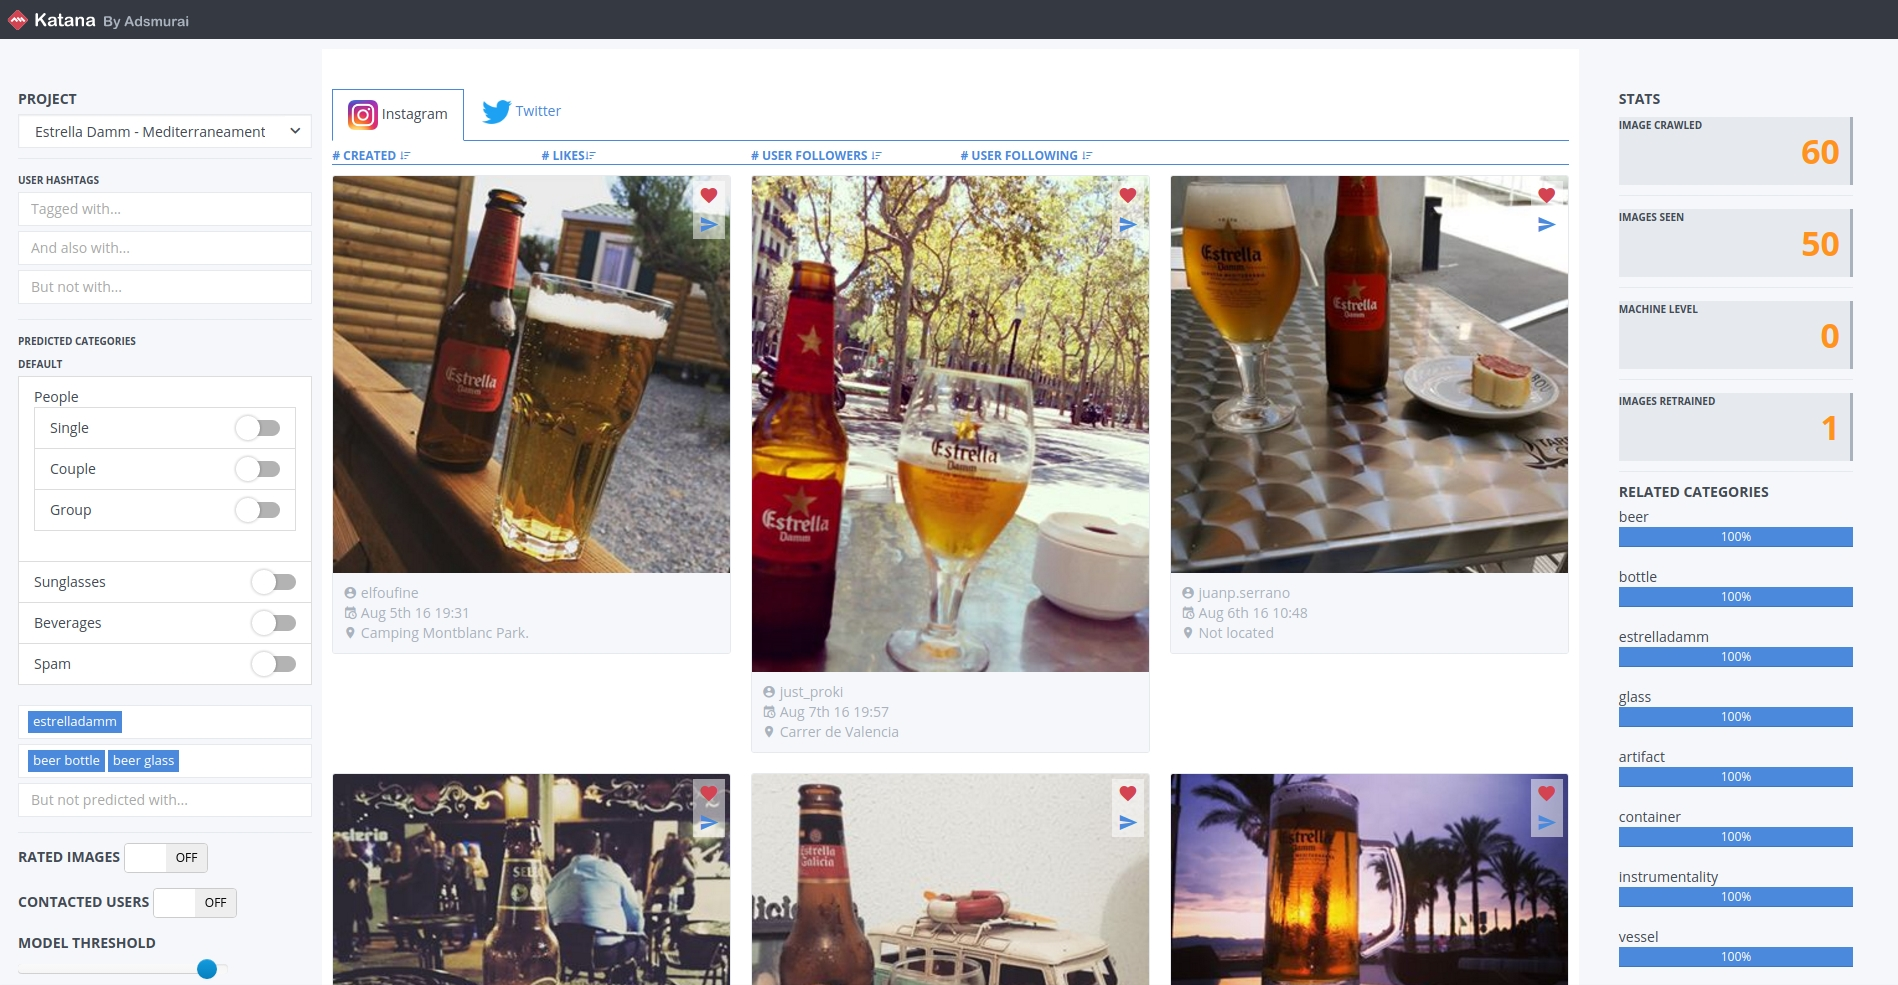
\includegraphics[width=3.0in]{Figs/ui1}}
%\caption{Screenshot of the user interface of the system, where users can navigate, search and select images from the database.} 
%\label{fig:ui}
%\end{center}
%\end{figure}





%********************************** %Second Section  *************************************
\section{Goals} %Section - 1.2


In this thesis, our general goal is to improve some techniques currently applied for automatically annotating photos posted by social media users. The generated annotations facilitate searching, filtering and analyzing user-generated content (UGC). We will apply scene-based and object-based image recognition techniques to extend the metadata originally present in the images with tags that describe their visual content. In order to reach state-of-the-art precission values we will employ CNNs. Performing these tasks in the UGC scenario implies some problems that are currently constraining their applicability to commercial systems. The specific goals of the project, that aim solving or mitigating some of these problems, are the following:

\begin{itemize} 
\item
Development of an efficient and scalable solution to enable complex image recogition pipelines for automatic UGC curation, where multiple CNN-based classifiers and object detectors can be chained in a graph fashion. The resulting solution must provide the necessary throughtput under reasonable cost assumptions, and must be able to scale. 
\item
Development of novel UGC-specific scene-based and object-based image recognition models, including but not limited to, a complete set of Instagram spam image detection models. 
\item
Development of a solution for the scalable training of on-demand custom classifiers and object detectors (e.g. company logos). Because of the particularities of these models, the resulting solution need to minimize training times and to be able to deal with small datasets. 
\end{itemize} 



\nomenclature[z-DKT]{DKT}{Draft Kiss Tumble}
\nomenclature[z-PPC]{PPC}{Particles per cell}
%!TEX root = ../thesis.tex
%*******************************************************************************
%****************************** Second Chapter *********************************
%*******************************************************************************

\chapter{State of the art}

\ifpdf
    \graphicspath{{Chapter2/Figs/Raster/}{Chapter2/Figs/PDF/}{Chapter2/Figs/}}
\else
    \graphicspath{{Chapter2/Figs/Vector/}{Chapter2/Figs/}}
\fi


\section[Short title]{Image recognition}

\subsection{Deep Convolutional Neural Networks}

\subsection{Classification}

\subsection{Object detection}

\section{Transfer Learning}

\section{Distributed training}





%!TEX root = ../thesis.tex
%*******************************************************************************
%****************************** Third Chapter **********************************
%*******************************************************************************
\chapter{Methodology}

% **************************** Define Graphics Path **************************
\ifpdf
    \graphicspath{{Chapter3/Figs/Raster/}{Chapter3/Figs/PDF/}{Chapter3/Figs/}}
\else
    \graphicspath{{Chapter3/Figs/Vector/}{Chapter3/Figs/}}
\fi

\section{Project phases}
We aim to address all the above mentioned goals by setting out following stages:

\paragraph{Phase 1: Development of novel UGC-specific image recognition models}

Select the proper CNN setup, acquire and preprocess the data and train a set of UGC-specific scene-based and object-based image recognition models, including a complete set of Instagram spam image detection models. Evaluate the performance and scalability of the combined execution of the resulting classifiers and detectors in real-time. Develop strategies that enable improving the performance and scalability of the solution. Evaluate the suitability of the solution when applied to custom models that need to be trained on-demand with small datasets.

\paragraph{Phase 2: Development of an arquitecture to enable complex image recogition pipelines for automatic UGC curation}

Taking as a starting point the setup resulting from Phase 1, it will be developed an efficient and scalable solution to enable chaining multiple classifiers and object detectors in a graph fashion. The resulting architecture will enable the definition of more complex image recogition pipelines for automatic UGC curation. 

\paragraph{Phase 3: Evaluation of the performance and scalability of the obtained solution enabling complex image recogition pipelines in a real scenario}
Define a real scenario and evaluate the performance and scalability of the results of Phase 2 under stress conditions. Examine the impact of different configurations and derive conclusions aiming to pave the way towards systematic and optimized methodologies for automatic UGC curation.


%%%%%%%%%%%%%%%%%%%%%%%%%%%%%%%%%%%%%%%%%%%%%%%%%%%%%%%%%%%%%%%%%%%%%%%%%%%%%%%%%%%%%%%%%%%%%%
%%%%%%%%%%%%%%%%%%%%%%%%%%%%%%%%%%%%%%%%%%%%%%%%%%%%%%%%%%%%%%%%%%%%%%%%%%%%%%%%%%%%%%%%%%%%%%
\section{Associated work plan}

I plan to finish my Ph.D in a total of three years. A tentative work plan of my future activities can be found in Figure \ref{gantt}. 

\begin{landscape}

\begin{figure}[b] 
\centering    

\includegraphics[width=1.0\textwidth]{minion}
\caption[Minion]{Here you can place the GANTT diagram as an image}
\label{gantt}
\end{figure}

\end{landscape}


- J1: This publication will describe the ..TODO.\\
- C2: This publication will evaluate ...TODO...\\
- C3 : This publication will detail...TODO.\\
- J2: This publication will summarize previous contributions on a real scenario...\\


\section{Completed activities}
In this last year, the first six months have been principally spent studying the topic and having theoretical research. Then I implemented ..... 

[DESCRIBE HERE THE WORK WITH SPARK4MN + DL4J. CLARIFY WHEN THE TESTS FINISHED (WHEN YOUR ACCOUNT WAS CLOSED) ]


\section{Resources}

\subsection{Data}

[TODO. Clarify that enven if the public API will change you still have the enough data in a save place]

\subsection{Hardware}

[TODO. Mention Adsmurai machines and also machines from the CAP research group.]

%\include{Chapter4/chapter4}
%\include{Chapter5/chapter5}
%\include{Chapter6/chapter6}
%\include{Chapter7/chapter7}



% ********************************** Back Matter *******************************
% Backmatter should be commented out, if you are using appendices after References
%\backmatter

% ********************************** Bibliography ******************************
\begin{spacing}{0.9}

% To use the conventional natbib style referencing
% Bibliography style previews: http://nodonn.tipido.net/bibstyle.php
% Reference styles: http://sites.stat.psu.edu/~surajit/present/bib.htm

\bibliographystyle{apalike}
%\bibliographystyle{unsrt} % Use for unsorted references  
%\bibliographystyle{plainnat} % use this to have URLs listed in References
\cleardoublepage
\bibliography{References/references} % Path to your References.bib file


% If you would like to use BibLaTeX for your references, pass `custombib' as
% an option in the document class. The location of 'reference.bib' should be
% specified in the preamble.tex file in the custombib section.
% Comment out the lines related to natbib above and uncomment the following line.

%\printbibliography[heading=bibintoc, title={References}]


\end{spacing}

% ********************************** Appendices ********************************

%\begin{appendices} % Using appendices environment for more functunality

%%!TEX root = ../thesis.tex
% ******************************* Thesis Appendix A ****************************
\chapter{How to install \LaTeX} 

\section*{Windows OS}

\subsection*{TeXLive package - full version}
\begin{enumerate}
\item	Download the TeXLive ISO (2.2GB) from\\
\href{https://www.tug.org/texlive/}{https://www.tug.org/texlive/}
\item	Download WinCDEmu (if you don't have a virtual drive) from \\
\href{http://wincdemu.sysprogs.org/download/}
{http://wincdemu.sysprogs.org/download/}
\item	To install Windows CD Emulator follow the instructions at\\
\href{http://wincdemu.sysprogs.org/tutorials/install/}
{http://wincdemu.sysprogs.org/tutorials/install/}
\item	Right click the iso and mount it using the WinCDEmu as shown in \\
\href{http://wincdemu.sysprogs.org/tutorials/mount/}{
http://wincdemu.sysprogs.org/tutorials/mount/}
\item	Open your virtual drive and run setup.pl
\end{enumerate}

or

\subsection*{Basic MikTeX - \TeX~ distribution}
\begin{enumerate}
\item	Download Basic-MiK\TeX (32bit or 64bit) from\\
\href{http://miktex.org/download}{http://miktex.org/download}
\item	Run the installer 
\item	To add a new package go to Start >> All Programs >> MikTex >> Maintenance (Admin) and choose Package Manager
\item	Select or search for packages to install
\end{enumerate}

\subsection*{TexStudio - \TeX~ editor}
\begin{enumerate}
\item	Download TexStudio from\\
\href{http://texstudio.sourceforge.net/\#downloads}
{http://texstudio.sourceforge.net/\#downloads} 
\item	Run the installer
\end{enumerate}

\section*{Mac OS X}
\subsection*{MacTeX - \TeX~ distribution}
\begin{enumerate}
\item	Download the file from\\
\href{https://www.tug.org/mactex/}{https://www.tug.org/mactex/}
\item	Extract and double click to run the installer. It does the entire configuration, sit back and relax.
\end{enumerate}

\subsection*{TexStudio - \TeX~ editor}
\begin{enumerate}
\item	Download TexStudio from\\
\href{http://texstudio.sourceforge.net/\#downloads}
{http://texstudio.sourceforge.net/\#downloads} 
\item	Extract and Start
\end{enumerate}


\section*{Unix/Linux}
\subsection*{TeXLive - \TeX~ distribution}
\subsubsection*{Getting the distribution:}
\begin{enumerate}
\item	TexLive can be downloaded from\\
\href{http://www.tug.org/texlive/acquire-netinstall.html}
{http://www.tug.org/texlive/acquire-netinstall.html}.
\item	TexLive is provided by most operating system you can use (rpm,apt-get or yum) to get TexLive distributions
\end{enumerate}

\subsubsection*{Installation}
\begin{enumerate}
\item	Mount the ISO file in the mnt directory
\begin{verbatim}
mount -t iso9660 -o ro,loop,noauto /your/texlive####.iso /mnt
\end{verbatim}

\item	Install wget on your OS (use rpm, apt-get or yum install)
\item	Run the installer script install-tl.
\begin{verbatim}
	cd /your/download/directory
	./install-tl
\end{verbatim}
\item	Enter command `i' for installation

\item	Post-Installation configuration:\\
\href{http://www.tug.org/texlive/doc/texlive-en/texlive-en.html\#x1-320003.4.1}
{http://www.tug.org/texlive/doc/texlive-en/texlive-en.html\#x1-320003.4.1} 
\item	Set the path for the directory of TexLive binaries in your .bashrc file
\end{enumerate}

\subsubsection*{For 32bit OS}
For Bourne-compatible shells such as bash, and using Intel x86 GNU/Linux and a default directory setup as an example, the file to edit might be \begin{verbatim}
edit $~/.bashrc file and add following lines
PATH=/usr/local/texlive/2011/bin/i386-linux:$PATH; 
export PATH 
MANPATH=/usr/local/texlive/2011/texmf/doc/man:$MANPATH;
export MANPATH 
INFOPATH=/usr/local/texlive/2011/texmf/doc/info:$INFOPATH;
export INFOPATH
\end{verbatim}
\subsubsection*{For 64bit OS}
\begin{verbatim}
edit $~/.bashrc file and add following lines
PATH=/usr/local/texlive/2011/bin/x86_64-linux:$PATH;
export PATH 
MANPATH=/usr/local/texlive/2011/texmf/doc/man:$MANPATH;
export MANPATH 
INFOPATH=/usr/local/texlive/2011/texmf/doc/info:$INFOPATH;
export INFOPATH

\end{verbatim}



%\subsection{Installing directly using Linux packages} 
\subsubsection*{Fedora/RedHat/CentOS:}
\begin{verbatim} 
sudo yum install texlive 
sudo yum install psutils 
\end{verbatim}


\subsubsection*{SUSE:}
\begin{verbatim}
sudo zypper install texlive
\end{verbatim}


\subsubsection*{Debian/Ubuntu:}
\begin{verbatim} 
sudo apt-get install texlive texlive-latex-extra 
sudo apt-get install psutils
\end{verbatim}

%\include{Appendix2/appendix2}

%\end{appendices}

% *************************************** Index ********************************
\printthesisindex % If index is present

\end{document}
